\graphicspath{{members/tf/figures/}}

\subsection{Pipeline A (sollte schon bei Saman anfgangen)}
\input{members/tf/authors}
\subsubsection{Area transition}
In previous steps we used clustering to estimate the fraction if pixels in the image from above that dosplay leave surface. But this value is only a fraction and no area measure jet.\\
To translate that fraction into an area we have to find the total area that the camera observes first. To do that we take a look at the camera setup again. \ref{fig:setupAbove}
   \begin{figure}[H]
       \centering
       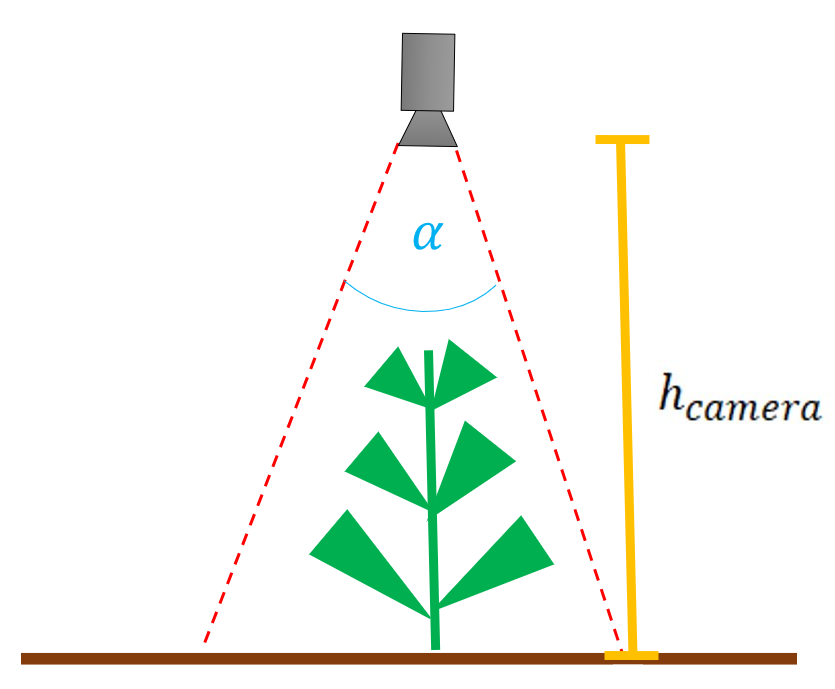
\includegraphics[scale=0.6]{setupAbove.PNG}
       \caption{Setup of the camera above the plant. $\alpha$ denotes the lense angle in which the camera captures the picture. $\alpha$ and $h_{Camera}$ are known.}
       \label{fig:setupAbove}
   \end{figure}{}
By only looking at half of the cone that the camera covers we can spot a triangle with a $90^{\circ}$ angle. Furthermore the height of the trianlge is $h_{Camera}$, the angle in the upper corner is $\frac{\alpha}{2}$ and the bottom side has a length of half the width of the observed area. The width of the observed area, calculated from the triangle needs to be squared, to get the area of the squared image:\\
$$A_{Camera} = (2\cdot h_{Camera}\cdot tan(\frac{\alpha}{2}))^2$$
$A_{Camera}$ only needs to be calculated once, as long as the camera parameters don't change. To calculate the area of the observed green, we simply multiply the captured area of the camera with the fraction $p_{Green}$ calculated by the clustering: 
$$A_{Observed} = p_{green}\cdot A_{Camera}$$
\textbf{Note:} This whole process works as long as the camera is set as supposed. A tilted camera would break the results since the used triangle would no longer have a $90^{\circ} angle. A tilted camera might also unintentionally capture adjacent plants.\\
\textbf{Model:} The observed plants are relatively small (max 40cm) in relation to the height of the camera (min 2m). Hence the plants can be considered to be flat on the ground, without changing the visible area. This assumption breaks when the plants grow much larger than expected. However this is pretty uncommon and can be therfore be neglected.
\subsubsection{Tilt angle correction}
The area calculated in the previous section represents the green area seen from above, which is not the area of the leaves in the canopy we are searching for. That's because the leaves aren't aligned horizontal but tilted and therefore their size is not perfectly captured as seen in \ref{fig:tiltedLeaves}. We have to add a correction to the obseved area to estimate the canopy area.\\
   \begin{figure}[H]
       \centering
       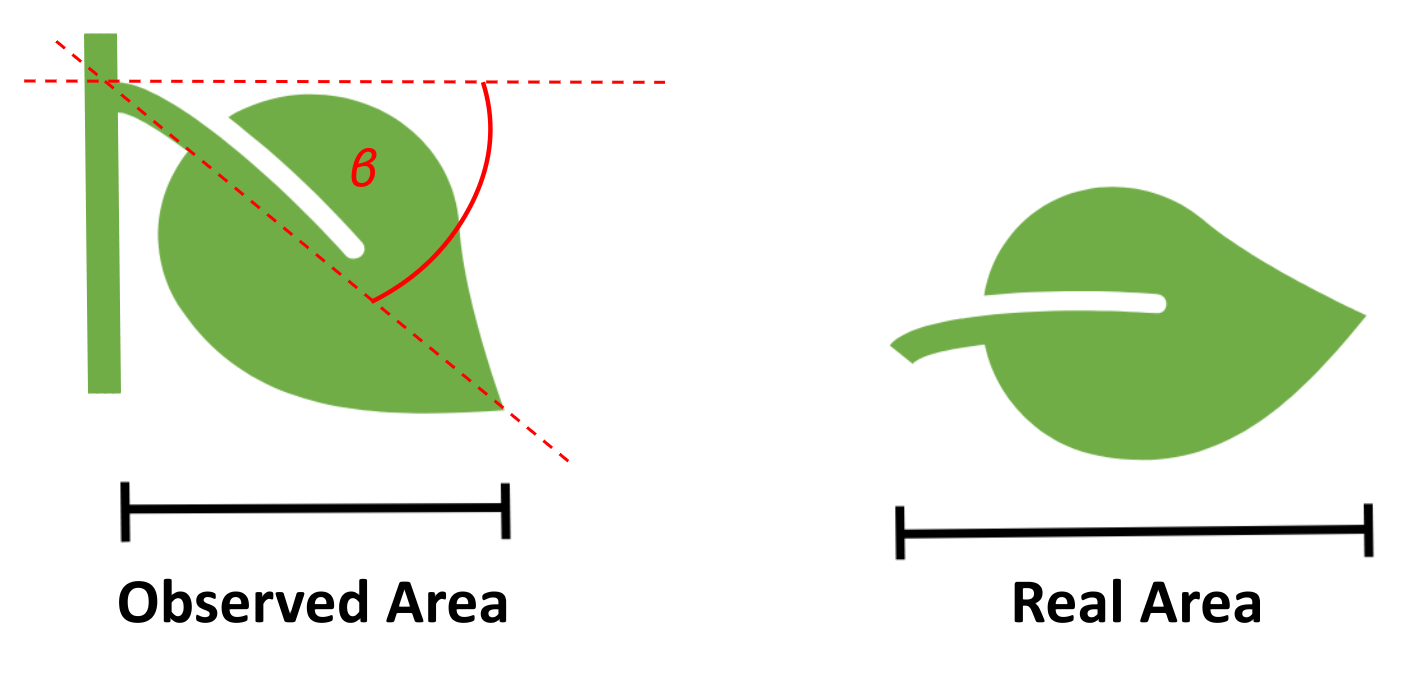
\includegraphics[scale=0.6]{tiltedLeaf.PNG}
       \caption{Sideview comparision of an untilted and a tilted leaf. The captured area from above reduces as a leaf gets tilted by an angle $\beta$.}
       \label{fig:tiltedLeaf}
   \end{figure}{}
The single leaves are assumed to be uncurved planes, therefore the observed area, the real area and the tilt angle $\beta$ form a $90^{\circ}$ triangle in the 2D sideview. Hence:
$$A_{Canopy} \approx \frac{A_{Observed}}{\arccos \langle |\beta |\rangle }$$
the absolute value of $\beta$ is used in this formula, because wether the tilting is upwards and downwards does not effect the visible area. furthermore the mean of $\beta$ is used, since the single tilt angles of the leaves are unknown and hard to estimate. That mean denotes the mean over all plants, not just a single one. However $\langle |\beta |\rangle$ is still hard to estimate, therefore $\arccos \langle |\beta |\rangle$ is replaced by a parameter that will be trained once the model is in use.\\
\textbf{Model: } The leaves are modeled as uncurved planes, which is most likely not true. Nevertheless the transform described in this section is expected to work, because the trained factor is will not only be trained to correct tiltangles but also curvature of the leaves. Using the model will show whether a linear model can learn this transformation. Assuming that each leaf is scaled by a factor, a linear model should do just fine. Coverage of leaves, which might also occure with adjacent leaves and affect the observed area will be discussed in section \ref{section:EstLAI}.
\subsection{Pipeline B}
\input{members/tf/authors}
\subsubsection{Height estimation setup}
\subsubsection{Estimating top of plant}
\subsubsection{Height estimation}
\subsection{Estimating LAI}
\label{section:EstLAI}
Beachte Überdeckungen innerhalb einer Ebene
\subsection{Yield prediction}
Lorem ipsum dolor sit amet, consetetur sadipscing elitr, sed diam nonumy eirmod tempor invidunt ut labore et dolore magna aliquyam erat, sed diam voluptua. At vero eos et accusam et justo duo dolores et ea rebum. Stet clita kasd gubergren, no sea takimata sanctus est Lorem ipsum dolor sit amet. Lorem ipsum dolor sit amet, consetetur sadipscing elitr, sed diam nonumy eirmod tempor invidunt ut labore et dolore magna aliquyam erat, sed diam voluptua. At vero eos et accusam et justo duo dolores et ea rebum. Stet clita kasd gubergren, no sea takimata sanctus est Lorem ipsum dolor sit amet. Lorem ipsum dolor sit amet, consetetur sadipscing elitr, sed diam nonumy eirmod tempor invidunt ut labore et dolore magna aliquyam erat, sed diam voluptua. At vero eos et accusam et justo duo dolores et ea rebum. Stet clita kasd gubergren, no sea takimata sanctus est Lorem ipsum dolor sit amet.

Duis autem vel eum iriure dolor in hendrerit in vulputate velit esse molestie consequat, vel illum dolore eu feugiat nulla facilisis at vero eros et accumsan et iusto odio dignissim qui blandit praesent luptatum zzril delenit augue duis dolore te feugait nulla facilisi. Lorem ipsum dolor sit amet, consectetuer adipiscing elit, sed diam nonummy nibh euismod tincidunt ut laoreet dolore magna aliquam erat volutpat.
